\documentclass{report}
% PACKAGES %
\usepackage[english]{} % Sets the language
\usepackage[margin=2cm]{geometry} % Sets the margin size
\usepackage{graphicx} % Enhanced package for including graphics/figures
\usepackage{float} % Allows figures and tables to be floats
\usepackage{amsmath} % Enhanced math package prepared by the American Mathematical Society
\usepackage{amssymb} % AMS symbols package
\usepackage{breqn} % Allows equation breaking over multiple lines
\usepackage{bm} % Allows you to use \bm{} to make any symbol bold
\usepackage{verbatim} % Allows you to include code snippets
\usepackage{setspace} % Allows you to change the spacing between lines at different points in the document
\usepackage{parskip} % Allows you alter the spacing between paragraphs
\usepackage{multicol} % Allows text division into multiple columns
\usepackage{units} % Allows fractions to be expressed diagonally instead of vertically
\usepackage{booktabs,multirow,multirow} % Gives extra table functionality
\usepackage{enumerate}
\newcommand{\tab}{\-\hspace{1.5cm}}

% Set path to figure image files
\graphicspath{ {fig/} }

\begin{document}

\begin{center}
\textbf{\large Nuclear Engineering 150 -- Discussion Section}\\ 
\textbf{Team Exercise Solutions \#1}

\-\\
{\small *Problems 1 \& 2 borrowed from Nuclear Engineering 101 homework problem sets, Fall 2016}
\end{center}


%%%%%%%%%%%%%%%%%%%%%%%%%%%%%%%%%% PROBLEM 1 %%%%%%%%%%%%%%%%%%%%%%%%%%%%%%%%%%
\section*{Problem 1}
The radioactive isotope $^{233}$Pa can be produced following neutron capture by $^{232}$Th when the resulting $^{233}$Th decays to $^{233}$Pa. In the neutron flux of a typical reactor, neutron capture in 1 g of $^{232}$Th produces $^{233}$Th at of a rate of $2.0 \times 10^{11}\text{ s}^{-1}$.
\begin{enumerate}[a)]
\item What are the activities (in Ci) of $^{233}$Th and $^{233}$Pa after this sample is irradiated for 1.5 hours?
\item The sample is then placed in storage with no further irradiation so that the $^{233}$Th can decay away. What are
the activities (in Ci) of $^{233}$Th and $^{233}$Pa after 48 hours of storage?
\item The decay of $^{233}$Pa results in $^{233}$U, which is also radioactive. After the above sample has been stored for 1 year what is the $^{233}$U activity in Ci? (Hint: it should not be necessary to set up an additional differential equation to find the $^{233}$U activity.)
\end{enumerate}

\begin{table}[htbp]
	\centering
	\begin{tabular}{|c|c|}
			\hline
			Nucleus		&	Half-life \\
			\hline
			$^{233}$Th	&  $22.3$ min\\
			$^{233}$Pa	&  $27.0$ days\\
			$^{233}$U	&  $1.592 \times 10^5$ yr\\
			\hline
	\end{tabular}
	\label{tab:design-specs}
\end{table}
\begin{center}$1\text{ Ci} = 3.7 \times 10^{10}\text{ s}^{-1}$\end{center}



\section*{Problem 1 Solution}


For all parts of this problem, let $R$ be the rate of neutron capture by 1 g of $^{232}$Th, $2.0 \times 10^{11} \;\text{s}^{-1}$.\\

\begin{enumerate}[a)]

\item

First, convert all half-lives and irradiation times to seconds for consistency.\\ 
\-\\
\tab $\lambda_{\text{Th}} = \frac{\ln{2}}{1338\text{s}} = 5.18\times10^{-4}\text{s}^{-1}$; \tab $\lambda_{\text{Pa}}=\frac{\ln{2}}{2332800s}=2.971\times10^{-7}\text{s}^{-1}$; \tab 1.5 hr = 5400 s\\

\textbf{Thorium-233}\\
\-\\
The rate of change of the quantity of $^{233}$Th, $\frac{dN_{\text{th}}}{dt}$ is given by the production rate of $^{233}$Th, $R$, minus the decay rate (activity) of $^{233}$Th, $\lambda_{\text{Th}}N_{\text{Th}}$.
$$\frac{dN_{\text{Th}}}{dt} = R - \lambda_{\text{Th}}N_{\text{Th}}$$
We manipulate the equation so that the left side is only dependent on $N_{\text{Th}}$ and the right side is only dependent on $dt$. Then integrate:
$$\int{\frac{dN_{\text{Th}}}{R-\lambda_{\text{Th}}N_{\text{Th}}}} = \int{dt}$$
$$\frac{-1}{\lambda_{\text{Th}}}[\ln(R-\lambda_{\text{Th}}N_{\text{Th}})] = t + C,\quad C=\text{const.}$$
$$R-\lambda_{\text{Th}}N_{\text{Th}} = e^{-\lambda_{\text{Th}}t -\lambda_{\text{Th}}C} = e^{-\lambda_{\text{Th}}t} e^{-\lambda_{\text{Th}}C}$$
We note that since $C$ is an arbitrary constant, we could also say $e^{-\lambda_{\text{Th}}C}$ is an arbitrary constant, and just call it $C$ instead.
$$ R-\lambda_{\text{Th}}N_{\text{Th}} = Ce^{-\lambda_{\text{Th}}t} $$
We solve for $N_{\text{Th}}$ (explicitly including $N_{\text{Th}}$'s dependence on $t$), and get
$$ N_{\text{Th}}(t) = \frac{R - Ce^{-\lambda_{\text{Th}}t}}{\lambda_{\text{Th}}} .$$
At $t=0,\; N_{\text{Th}}(0) = \frac{R - C}{\lambda_{\text{Th}}}=0,$ since no $^{233}$\text{Th} has been formed. We find $C= R$, and use this in the general equation:
$$ N_{\text{Th}}(t) = R\frac{1 - e^{-\lambda_{\text{Th}}t}}{\lambda_{\text{Th}}}. $$
With this function of $N_{\text{Th}}$, we can determine the activity as a function of time, knowing that
$$ \mathcal{A}_{\text{Th}}(t) = \lambda_{\text{Th}}N_{\text{Th}}(t). $$
Substituting, we find
$$ \mathcal{A}_{\text{Th}}(t) = R(1-e^{-\lambda_{\text{Th}}t}) .$$
Using the numerical values for $R$, $\lambda_{\text{Th}}$, and $t$,
$$ \mathcal{A}_{\text{Th}}(1.5\text{ hr}) =(2.0\times10^{11}s^{-1})(1-e^{(-5.18\times10^{-4}\text{s}^{-1})(5400s)}) $$
$$ \mathcal{A}_{\text{Th}}(1.5\text{ hr}) = 1.878\times10^{11}\text{ Bq} .$$
Finally, we convert this to Curies,
$$\boxed{ \mathcal{A}_{\text{Th}}(1.5\text{ hr}) = 5.076\text{ Ci} }.$$

\textbf{Protactinium-233}\\
\-\\
We follow a similar procedure for $^{233}$Pa, noting that the production rate of $^{233}$Pa is just the activity of $^{233}$Th as it decays into $^{233}$Pa, $\mathcal{A}_{\text{Th}}$.
$$\frac{dN_{\text{Pa}}}{dt} = \mathcal{A}_{\text{Th}} - \lambda_{\text{Pa}}N_{\text{Pa}}$$
From above, we can substitue our function for $\mathcal{A}_{\text{Th}}(t)$,
$$\frac{dN_{\text{Pa}}}{dt} = R(1-e^{-\lambda_{\text{Th}}t}) - \lambda_{\text{Pa}}N_{\text{Pa}}$$
We note here that we cannot separate both sides to be dependent only on a single differential, so we must try a different method of integration. We will use integrating factors. We do, however start in a similar fashion: collecting the terms dependent on $N_{\text{Pa}}$ on the same side.
$$ \frac{dN_{\text{Pa}}}{dt}+\lambda_{\text{Pa}}N_{\text{Pa}} = R(1-e^{-\lambda_{\text{Th}}t}) $$
The method of integrating factors suggests that we multiply both sides by an arbitrary exponential. We will use $e^{\lambda_{\text{Pa}}t}$.
$$ e^{\lambda_{\text{Pa}}t}\frac{dN_{\text{Pa}}}{dt} + \lambda_{\text{Pa}}e^{\lambda_{\text{Pa}}t}N_{\text{Pa}} = e^{\lambda_{\text{Pa}}t}R(1-e^{-\lambda_{\text{Th}}t}) $$
We can now observe that the left side of the equation appears to be the result of the product rule when the derivative with respect to time is taken of the expression $e^{\lambda_{\text{Pa}}t}N_{\text{Pa}}$. We can then write the equation as
$$\frac{d}{dt}(e^{\lambda_{\text{Pa}}t}N_{\text{Pa}}) = e^{\lambda_{\text{Pa}}t}R(1-e^{-\lambda_{\text{Th}}t})$$
Moving the $dt$ term to the right side of the equation and using the distributive property, we have
$$ d(e^{\lambda_{\text{Pa}}t}N_{\text{Pa}}) = R(e^{\lambda_{\text{Pa}}t}-e^{\lambda_{\text{Pa}}t}e^{-\lambda_{\text{Th}}t})dt .$$
We integrate both sides,
$$ \int{d(e^{\lambda_{\text{Pa}}t}N_{\text{Pa}})} = \int{ R(e^{\lambda_{\text{Pa}}t}-e^{\lambda_{\text{Pa}}t-\lambda_{\text{Th}}t})dt}, $$
separate the integral on the right side,
$$ e^{\lambda_{\text{Pa}}t}N_{\text{Pa}} = R\int{ e^{\lambda_{\text{Pa}}t}dt}-R\int{e^{(\lambda_{\text{Pa}}-\lambda_{\text{Th}})t}dt} $$
and find
$$e^{\lambda_{\text{Pa}}t}N_{\text{Pa}} = \frac{R}{\lambda_{\text{Pa}}}e^{\lambda_{\text{Pa}}t}-\frac{R}{\lambda_{\text{Pa}}-\lambda_{\text{Th}}}e^{(\lambda_{\text{Pa}}-\lambda_{\text{Th}})t} +\;C,\; C=\text{const.}$$
Now we factor out the integrating factor back out from both sides and note the explicit time dependence of $N_{\text{Pa}}$,
$$N_{\text{Pa}}(t) = \frac{R}{\lambda_{\text{Pa}}}-\frac{R}{\lambda_{\text{Pa}}-\lambda_{\text{Th}}}e^{-\lambda_{\text{Th}}t}+Ce^{-\lambda_{\text{Pa}}t}$$
At $t=0$,
$$ N_{\text{Pa}}(0) = \frac{R}{\lambda_{\text{Pa}}}-\frac{R}{\lambda_{\text{Pa}}-\lambda_{\text{Th}}}+C = 0, $$
 since no $^{233}$\text{Pa} has been formed. Solving for $C$, we find $C = \frac{R}{\lambda_{\text{Pa}}-\lambda_{\text{Th}}}-\frac{R}{\lambda_{\text{Pa}}}$. We plug this back into our equation above, and have the solution for $N_{\text{Pa}}(t)$:
$$N_{\text{Pa}}(t) = \frac{R}{\lambda_{\text{Pa}}}-\frac{R}{\lambda_{\text{Pa}}-\lambda_{\text{Th}}}e^{-\lambda_{\text{Th}}t}+\left( \frac{R}{\lambda_{\text{Pa}}-\lambda_{\text{Th}}}-\frac{R}{\lambda_{\text{Pa}}} \right)e^{-\lambda_{\text{Pa}}t}$$
and simplifying
$$ N_{\text{Pa}}(t) = \frac{R}{\lambda_{\text{Pa}}}(1-e^{\lambda_{\text{Pa}}t})+ \left(\frac{R}{\lambda_{\text{Pa}}-\lambda_{\text{Th}}}\right)(e^{-\lambda_{\text{Pa}}t}-e^{-\lambda_{\text{Th}}t}) .$$
With this function of $N_{\text{Pa}}$, we can determine the activity as a function of time, knowing that
$$ \mathcal{A}_{\text{Pa}}(t) = \lambda_{\text{Pa}}N_{\text{Pa}}(t) .$$
Substituting, we find
$$ \mathcal{A}_{\text{Pa}}(t) = R(1-e^{-\lambda_{\text{Pa}}t})+ \left(\frac{R \, \lambda_{\text{Pa}}}{\lambda_{\text{Pa}}-\lambda_{\text{Th}}}\right)(e^{-\lambda_{\text{Pa}}t}-e^{-\lambda_{\text{Th}}t}) .$$
Using the numerical values for $R$, $\lambda_{\text{Th}}$, $\lambda_{\text{Pa}}$, and $t$,
\begin{dmath*}
\mathcal{A}_{\text{Pa}}(1.5\text{ hr}) = (2.0\times10^{11}\text{ s}^{-1})\left(1-e^{(-2.971\times10^{-7}\text{s}^{-1})(5400\text{s})}\right)+ \left(\frac{2.0\times10^{11}\text{ s}^{-1}(2.791\times10^{-7}\text{s}^{-1})}{2.971\times10^{-7}\text{s}^{-1}-5.18\times10^{-4}\text{s}^{-1}}\right)\left(e^{(-2.971\times10^{-7}\text{s}^{-1})(5400\text{s})}-e^{(-5.18\times10^{-4}\text{s}^{-1})(5400\text{s})}\right)
\end{dmath*}
$$ \mathcal{A}_{\text{Pa}}(1.5\text{ hr}) = 2.195 \times 10^{8}\text{ Bq} $$
Finally, we convert this to Curies, 
$$ \boxed{\mathcal{A}_{\text{Pa}}(1.5\text{ hr}) = 0.006\text{ Ci}}. $$

\item

Let's say that the 1.5 hour mark is now given by $t=t_0=1.5\text{ hr}$. We also note that 48 hours = 172,800 seconds.

\textbf{Thorium-233}\\
\-\\
Without irradiation, the rate of change of the quantity of $^{233}$Th is now just the decay rate. 
$$ \frac{dN_{\text{Th}}}{dt} = -\lambda_{\text{Th}}N_{\text{Th}} $$
We separate the equation and integrate, arriving at the standard exponential decay formula, now including the explicit time dependence.
$$ \int_{N_{\text{Th}}(t_0)}^{N_{\text{Th}}(t)} \frac{-dN_{\text{Th}}'}{\lambda_{\text{Th}}N_{\text{Th}}'} = \int_{t_0}^{t} dt' $$
$$ \frac{-1}{\lambda_{\text{Th}}}\left[ \ln{N_{\text{Th}}} \right]_{N_{\text{Th}(t_0)}}^{N_{\text{Th}}(t)} = \left[t'\right]_{t_0}^{t} $$
$$ \ln\frac{N_{\text{Th}}(t)}{N_{\text{Th}}(t_0)}  = -\lambda_{\text{Th}}(t-t_0) $$
$$ \frac{N_{\text{Th}}(t)}{N_{\text{Th}}(t_0)}  = e^{-\lambda_{\text{Th}}(t-t_0)} $$
and we have 
$$ N_{\text{Th}}(t) = N_{\text{Th}}(t_0) e^{-\lambda_{\text{Th}}\left(t-t_0\right)} $$
Given the definition of activity as $\mathcal{A} = \lambda N$ and noting $\lambda_{\text{Th}} N_{\text{Th}}(t_0) = \mathcal{A}_{\text{Th}}(t_0)$, we can write the activity of $^{233}$Th as
\begin{align*}
\mathcal{A}_{\text{Th}}(t)	&= \lambda_{\text{Th}} N_{\text{Th}}(t) \\
							&= \lambda_{\text{Th}} N_{\text{Th}}(t_0) e^{-\lambda_{\text{Th}}(t-t_0)} \\ 
							&= \mathcal{A}_{\text{Th}}(t_0) e^{-\lambda_{\text{Th}}(t-t_0)}
\end{align*}
Using the numerical values for $\lambda_{\text{Th}}$, $t$, and our answer from part (a) for the activity at $t_0=1.5$ hr, we find
$$ \mathcal{A}_{\text{Th}}(49.5\text{ hr}) = (5.076 \text{ Ci})e^{-5.18\times10^{-4}\text{s}^{-1} (172800\text{s})} $$
$$ \boxed{\mathcal{A}_{\text{Th}}(49.5\text{ hr}) = 6.787\times10^{-39}\text{ Ci}} $$

{\small Note: we could also have assumed that since 48 hours is many (more than 100) times longer than the half-life of $^{233}$Th, that the activity would be approximately zero.}
\-\\
\-\\

\textbf{Protactinium-233}\\
\-\\
We follow the example in part (a) for $^{233}$Pa, again using the activity of $^{233}$Th as the production rate of $^{233}$Pa.
$$ \frac{dN_{\text{Pa}}}{dt} = \mathcal{A}_{\text{Th}} - \lambda_{\text{Pa}}N_{\text{Pa}}. $$
We collect terms dependent on $N_{\text{Pa}}$ on one side,
$$ \frac{dN_{\text{Pa}}}{dt} + \lambda_{\text{Pa}}N_{\text{Pa}} = \mathcal{A}_{\text{Th}}(t_0) e^{-\lambda_{\text{Th}}(t-t_0)}, $$
multiply both sides by arbitrary exponential $e^{\lambda_{\text{Pa}}t}$,
$$ e^{\lambda_{\text{Pa}}t}\frac{dN_{\text{Pa}}}{dt} + \lambda_{\text{Pa}}e^{\lambda_{\text{Pa}}t}N_{\text{Pa}} = e^{\lambda_{\text{Pa}}t}\mathcal{A}_{\text{Th}}(t_0) e^{-\lambda_{\text{Th}}(t-t_0)}, $$
note that the left side is the result of the product rule when $\frac{d}{dt}$ is taken on $e^{\lambda_{\text{Pa}}t}N_{\text{Pa}}$
$$ \frac{d}{dt} (e^{\lambda_{\text{Pa}}t}N_{\text{Pa}}) = e^{\lambda_{\text{Pa}}t}\mathcal{A}_{\text{Th}}(t_0) e^{-\lambda_{\text{Th}}(t-t_0)}, $$
multiply by the differential, $dt$,
$$ d(e^{\lambda_{\text{Pa}}t}N_{\text{Pa}}) = e^{\lambda_{\text{Pa}}t}\mathcal{A}_{\text{Th}}(t_0) e^{-\lambda_{\text{Th}}(t-t_0)} dt ,$$
and rearrange,
$$ d(e^{\lambda_{\text{Pa}}t}N_{\text{Pa}}) = \mathcal{A}_{\text{Th}}(t_0) e^{(\lambda_{\text{Pa}} - \lambda_{\text{Th}})t + \lambda_{\text{Th}}t_0} dt .$$
Then we integrate,
$$ \int_{e^{\lambda_{\text{Pa}}t_0}N_{\text{Pa}}(t_0)}^{e^{\lambda_{\text{Pa}}t}N_{\text{Pa}}(t)} d(e^{\lambda_{\text{Pa}}t}N_{\text{Pa}}') = \mathcal{A}_{\text{Th}}(t_0)e^{\lambda_{\text{Th}}t_0} \int_{t_0}^{t} e^{(\lambda_{\text{Pa}} - \lambda_{\text{Th}})t'} dt' ,$$
and find,
$$ \left[e^{\lambda_{\text{Pa}}t}N_{\text{Pa}}'\right]_{e^{\lambda_{\text{Pa}}t_0}N_{\text{Pa}}(t_0)}^{e^{\lambda_{\text{Pa}}t}N_{\text{Pa}}(t)} = \frac{\mathcal{A}_{\text{Th}}(t_0)e^{\lambda_{\text{Th}}t_0}}{\lambda_{\text{Pa}}-\lambda_{\text{Th}}} \left[ e^{(\lambda_{\text{Pa}}-\lambda_{\text{Th}})t'}\right]_{t_0}^{t} $$
$$ e^{\lambda_{\text{Pa}}t}N_{\text{Pa}}(t) - e^{\lambda_{\text{Pa}}t_0}N_{\text{Pa}}(t_0) = \frac{\mathcal{A}_{\text{Th}}(t_0)e^{\lambda_{\text{Th}}t_0}}{\lambda_{\text{Pa}}-\lambda_{\text{Th}}} \left[ e^{(\lambda_{\text{Pa}}-\lambda_{\text{Th}})t} - e^{(\lambda_{\text{Pa}}-\lambda_{\text{Th}})t_0} \right] $$
Factoring out the integrating factor, 
$$ N_{\text{Pa}}(t) - e^{-\lambda_{\text{Pa}}(t - t_0)}N_{\text{Pa}}(t_0) = \frac{\mathcal{A}_{\text{Th}}(t_0)e^{\lambda_{\text{Th}}t_0}}{\lambda_{\text{Pa}}-\lambda_{\text{Th}}} \left[ e^{-\lambda_{\text{Th}}t} - e^{-\lambda_{\text{Pa}}t}e^{(\lambda_{\text{Pa}}-\lambda_{\text{Th}})t_0} \right] $$
and solve for $ N_{\text{Pa}}(t)$,
$$ N_{\text{Pa}}(t) = \frac{\mathcal{A}_{\text{Th}}(t_0)e^{\lambda_{\text{Th}}t_0}}{\lambda_{\text{Pa}}-\lambda_{\text{Th}}} \left[ e^{-\lambda_{\text{Th}}t} - e^{-\lambda_{\text{Pa}}t}e^{(\lambda_{\text{Pa}}-\lambda_{\text{Th}})t_0} \right] + e^{-\lambda_{\text{Pa}}(t-t_0)}N_{\text{Pa}}(t_0) .$$
Rearranging,
$$ N_{\text{Pa}}(t) = \frac{\mathcal{A}_{\text{Th}}(t_0)}{\lambda_{\text{Pa}}-\lambda_{\text{Th}}} \left[ e^{-\lambda_{\text{Th}}(t - t_0)} - e^{-\lambda_{\text{Pa}}(t-t_0)} \right] + e^{-\lambda_{\text{Pa}}(t - t_0)}N_{\text{Pa}}(t_0) .$$
and so
$$ N_{\text{Pa}}(t) = \frac{\mathcal{A}_{\text{Th}}(t_0)}{\lambda_{\text{Pa}}-\lambda_{\text{Th}}} e^{-\lambda_{\text{Th}}(t-t_0)} + \left( N_{\text{Pa}}(t_0) - \frac{\mathcal{A}_{\text{Th}}(t_0)}{\lambda_{\text{Pa}}-\lambda_{\text{Th}}} \right) e^{-\lambda_{\text{Pa}}(t-t_0)} $$
Given the definition of activity as $\mathcal{A} = \lambda N$ and noting $\lambda_{\text{Pa}} N_{\text{Pa}}(t_0) = \mathcal{A}_{\text{Pa}}(t_0)$, we can write the activity of $^{233}$Pa as
\begin{align*}
\mathcal{A}_{\text{Pa}}(t)	&= \lambda_{\text{Pa}} N_{\text{Pa}}(t) \\
							&=\lambda_{\text{Pa}} \left(\frac{\mathcal{A}_{\text{Th}}(t_0)}{\lambda_{\text{Pa}}-\lambda_{\text{Th}}} e^{-\lambda_{\text{Th}}(t-t_0)} + \left( N_{\text{Pa}}(t_0) - \frac{\mathcal{A}_{\text{Th}}(t_0)}{\lambda_{\text{Pa}}-\lambda_{\text{Th}}} \right) e^{-\lambda_{\text{Pa}}(t-t_0)}\right) \\
							&= \frac{\mathcal{A}_{\text{Th}}(t_0) \lambda_{\text{Pa}}}{\lambda_{\text{Pa}}-\lambda_{\text{Th}}} e^{-\lambda_{\text{Th}}(t-t_0)} + \left( \mathcal{A}_{\text{Pa}}(t_0) - \frac{\mathcal{A}_{\text{Th}}(t_0) \lambda_{\text{Pa}}}{\lambda_{\text{Pa}}-\lambda_{\text{Th}}} \right) e^{-\lambda_{\text{Pa}}(t-t_0)} \\
							&= \mathcal{A}_{\text{Pa}}(t_0) e^{-\lambda_{\text{Pa}}(t-t_0)} +  \frac{\mathcal{A}_{\text{Th}}(t_0) \lambda_{\text{Pa}}}{\lambda_{\text{Pa}}-\lambda_{\text{Th}}} \left( e^{-\lambda_{\text{Th}}(t-t_0)} - e^{-\lambda_{\text{Pa}}(t-t_0)} \right) \\
\end{align*}
Using the numerical values for $\lambda_{\text{Th}}$, $\lambda_{\text{Pa}}$, $t$, and our answer from part (a) for the activities at $t=t_0=1.5$ hr, we find
\begin{dmath*}
\mathcal{A}_{\text{Pa}}(49.5\text{ hr}) = (0.006\text{ Ci}) e^{-(2.971\times10^{-7}\text{s}^{-1})(172800s)} +  \frac{(5.076\text{ Ci}) (2.971\times10^{-7}\text{s}^{-1})}{2.971\times10^{-7}\text{s}^{-1}-5.18\times10^{-4}\text{s}^{-1}} \left( e^{-(5.18\times10^{-4}\text{s}^{-1})(172800s)} - e^{-(2.971\times10^{-7}\text{s}^{-1})(172800s)} \right)
\end{dmath*}
$$\boxed{ \mathcal{A}_{\text{Pa}}(49.5\text{ hr}) = 0.008\text{ Ci} }$$

\item 

Note that $\lambda_{\text{U}} = \frac{\ln 2}{5.024^{12}\text{s}} = 1.380\times10^{-13}\text{s}^{-1}$. 

In just one day, the probability that any given $^{233}$Th nucleus survives is
$$ P = e^{-\lambda_{\text{Th}}t_d} $$
$$ P = e^{-(5.18\times10^{-4}\text{ s}^{-1})(86,400\text{ s})} \approx 10^{-20} $$
We can therefore assume that each thorium nucleus produced in the reactor has decayed into $^{233}$Pa by the end of the first day of storage. (There were only about $10^{15}$ thorium nuclei produced in total).
The probability that any one of these $^{233}$Pa atoms remains after one year---assumed to be 364 more days---is
$$ P = e^{-\lambda_{\text{Pa}}(t_y-t_d)} $$
$$ P = e^{-(2.971\times10^{-7}\text{ s}^{-1})(31449600\text{ s})} = 8.752\times10^{-5}  $$
While this probability indicates that some $^{233}$Pa nuclei will remain after the year of storage, they hardly make up a substantial fraction of the originally produced set of nuclei. We can assume that in one year, virtually every nucleus of $^{233}$Th has decayed at least into $^{233}$U.  

For uranium-233 on the other hand, the probability of survival for a nucleus over a year is
$$ P = e^{-\lambda_{\text{U}}t_y} $$
$$ P = e^{-(1.380\times10^{-13})(31536000\text{ s})} $$
$$ P = 0.999996 $$
We see that while nearly every nucleus decays from $^{233}$Th into $^{233}$Pa and then into $^{233}$U, almost no nuclei seem to decay from $^{233}$U in the single year.
We can then use our simple formula for the activity of the uranium sample
$$ \mathcal{A}_{\text{U}} = \lambda_{\text{U}} N_{\text{U}}$$

Using our rate of production, there are $2.0\times10^{11}\text{ s}^{-1}*(3600\text{ s/hr}\times 1.5 \text{hr}) \approx 1.08\times10^{15}$ produced in the irradiation period. We will assume this is also equal to the number of nuclei of $^{233}$U present at the end of the 1 year storage period: $N_U \approx 10^{15}$. We can finally calculate the activity, as 
$$ \mathcal{A}_{\text{U}} = (1.380\times10^{-13}\text{s}^{-1})(1.08\times10^{15}) .$$
This is ${149.04}\text{ Bq}$ or 
$$\boxed{ 4.028\times10^{-9}\text{ Ci} }$$
\end{enumerate}


\newpage
%%%%%%%%%%%%%%%%%%%%%%%%%%%%%%%%%% PROBLEM 2 %%%%%%%%%%%%%%%%%%%%%%%%%%%%%%%%%%
\section*{Problem 2}

Use the following masses for parts (a) and (b):

\begin{table}[htbp]
	\centering
	\begin{tabular}{|c|c|}
			\hline
			Nucleus		&	Atomic Mass \\
			\hline
			n 			&	 1.008665 u \\
			$^{1}$H		& 	 1.007825 u \\
			$^{2}$H 	&	 2.014102 u \\
			$^{56}$Fe	&   55.934939 u \\
			$^{98}$Y 	&   97.922203 u \\
			$^{135}$I	&  134.910048 u \\
			$^{235}$U	&  235.043924 u \\
			\hline
	\end{tabular}
	\label{tab:design-specs}
\end{table}
\begin{center}$1\text{u} \cdot c^{2} = 931.502$ MeV\end{center}
\-\\
\begin{enumerate}[a)]
\item Calculate the $Q$-value of the reaction:
$$ ^{235}\text{U}\, + \,n \-\rightarrow\- ^{135}\text{I}\, + \,^{98}\text{Y}\, + \,3n $$
\item Calculate the average binding energy per nucleon (in MeV) of $^{2}$H, $^{56}$Fe, and $^{235}$U.
\end{enumerate}



\section*{Problem 2 Solution}

\begin{enumerate}[a)]

\item 

The $Q$-value of a reaction is given by:$$Q=[m(\text{x})+m(\text{X})-m(\text{y})-m(\text{Y})]c^{2}.$$

\begin{spacing}{1.75}	
$^{235}\text{\normalfont{U}}+n \rightarrow  \-\ ^{135}\text{\normalfont{I}}+ \! ^{98}\text{\normalfont{Y}}+3n$\\
	\tab $Q = [m(^{235}\text{\normalfont{U}})+m(n)-m(^{135}\text{\normalfont{I}})-m(^{98}\text{\normalfont{Y}})-3m(n)]c^{2}$\\
	\tab $Q = [235.043924\text{u}+1.008665\text{u}-134.910048\text{u}-97.922203\text{u}-3(1.008665\text{u})]c^{2}$\\
	\tab $Q = 0.194343\text{u} \cdot c^{2}$\\
	\tab $\boxed{Q = 181.031 \text{ MeV}}$ 
\end{spacing}


\item 

The binding energy $B(Z,A)$ for any nuclei can be found approximately from the equation:$$M(Z,A) = Zm(^{1}\text{H})+(A-Z)m_{n}-B(Z,A)/c^{2},$$ where $M(Z,A),\; Zm(^{1}\text{H})$ and $m_{n}$ are experimentally calculated values. Per nucleon, the binding energy can be expressed as: $$B_{A}(Z,A) = [Zm(^{1}\text{H})+(A-Z)m_{n}-M(Z,A)]c^{2}/A.$$

\begin{spacing}{1.75}

\textbf{$^{2}$H}\\
$B_{A}(1,2) = [m(^{1}\text{H})+(2-1)m_{n}-M(1,2)]c^{2}/2$\\
$B_{A}(1,2) = [(1.007825\text{u})+(1.008665\text{u})-(2.014102\text{u})]c^{2}/2$\\
$B_{A}(1,2) = 0.001194\text{u} \cdot c^{2}$\\
$\boxed{B_{A}(1,2) = 1.112\text{ MeV}}$\\
\textbf{$^{56}$Fe}\\
$B_{A}(26,56) = [26m(^{1}\text{H})+(56-26)m_{n}-M(26,56)]c^{2}/56$\\
$B_{A}(26,56) = [26(1.007825\text{u})+30(1.008665\text{u})-(55.934939\text{u})]c^{2}/56$\\
$B_{A}(26,56) = 0.009437\text{u} \cdot c^{2}$\\
$\boxed{B_{Z}(26,56) = 8.791\text{ MeV}}$\\
\textbf{$^{235}$U}\\
$B_{A}(92,235) = [92m(^{1}\text{H})+(235-92)m_{n}-M(92,235)]c^{2}/235$\\
$B_{A}(92,235) = [92(1.007825\text{u})+143(1.008665\text{u})-(235.043924\text{u})]c^{2}/235$\\
$B_{A}(92,235) = 0.00814924 u\text{u} \cdot c^{2}$\\
$\boxed{B_{Z}(92,235) = 7.591\text{ MeV}}$
\end{spacing}

\end{enumerate}



\newpage
%%%%%%%%%%%%%%%%%%%%%%%%%%%%%%%%%% PROBLEM 3 %%%%%%%%%%%%%%%%%%%%%%%%%%%%%%%%%%
\section*{Problem 3}

\begin{enumerate}[a)]
\item Solve the first order differential equation
$$ \frac{dy}{dx} + 3y = 0 $$
\item Solve the second order differential equation ($A$ and $B$ are constants)
$$ \frac{d^2 y}{dx^2} - A^2y = B $$
The boundary condition is $y(\pm\frac{1}{A}) = 0$.
\end{enumerate}



\section*{Problem 3 Solution}
\begin{enumerate}[a)]

\item 

\begin{align*}
\frac{dy}{dx}	&= -3y \\
\frac{dy}{y} 	& = -3\,dx \\
\int\frac{dy}{y}&= -3 \int \,dx \\
\ln y			&= -3 x + C \\
y				&= e^{-3x + C} \\
\end{align*}
$$\boxed{y = Ce^{-3x}}$$

\item 

Solve the second order differential equation
$$ \frac{d^2 y}{dx^2} - A^2y = B $$
For the homogeneous equation, $\frac{d^2 y}{dx^2} - A^2y = 0$, try $y_c = X_1 e^{Ax} + X_2 e^{-Ax}$ as the complementary solution ($X_1$ and $X_2$ are constants). Then
$$ \frac{d^2 y}{dx^2} = X_1 A^2 e^{Ax} + X_2 A^2 e^{-Ax} $$
and
$$ (X_1 A^2 e^{Ax} + X_2 A^2 e^{-Ax}) - A^2(X_1 e^{Ax} + X_2 e^{-Ax}) = 0 $$
$$ A^2 (X_1 e^{Ax} + X_2 e^{-Ax}) - A^2 (X_1 e^{Ax} + X_2 e^{-Ax}) = 0 $$

This is \underline{true}.

For the inhomogeneous equation, $\frac{d^2 y}{dx^2} - A^2y = B$, $y_P = -B/A^2$ is the only particular solution satisfying the equation. The general solution is the sum of the complementary and particular solutions, $y = y_c + y_p$. 
$$ y = X_1 e^{Ax} + X_2 e^{-Ax} - \frac{B}{A^2} $$
Now we can solve for $X_1$ and $X_2$. 
$$ y(\frac{1}{A}) = X_1 e^{A(\frac{1}{A})} + X_2 e^{-A(\frac{1}{A})} - \frac{B}{A^2} = 0 $$
and
$$ y(-\frac{1}{A}) = X_1 e^{A(-\frac{1}{A})} + X_2 e^{A(\frac{1}{A})} - \frac{B}{A^2} = 0 $$
We can note that in these two equations, $X_1$ and $X_2$ can be interchanged freely, and so must be equal. We will say, $X_1 = X_2 = X$. Then, we have
$$ 0 = X e^{A(-\frac{1}{A})} + X e^{A(\frac{1}{A})} - \frac{B}{A^2} $$
$$ 0 = X (e^{-1} + e^{1}) - \frac{B}{A^2} $$
$$ X = \frac{B}{A^2(\frac{1}{e} + e)} $$
The we plug this $X$ into the final solution, which gives
$$ y = \frac{B}{A^2(\frac{1}{e} + e)} (e^{Ax} + e^{-Ax}) - \frac{B}{A^2} $$
\end{enumerate}
Note that $e^{Ax} + e^{-Ax}$ is similar in form to $\cosh(Ax)$ which we could have also used to solve this problem.



\newpage
%%%%%%%%%%%%%%%%%%%%%%%%%%%%%%%%%% PROBLEM 4 %%%%%%%%%%%%%%%%%%%%%%%%%%%%%%%%%%
\section*{Problem 4}

Classify the following cross section plots. They are, in no particular order:
\begin{enumerate}[(1)]
\item $^{155}$Gd absorption
\item $^{235}$U fission
\item $^{238}$U absorption
\item $^{238}$U fission
\item $^{239}$Pu fission
\end{enumerate}

(a) 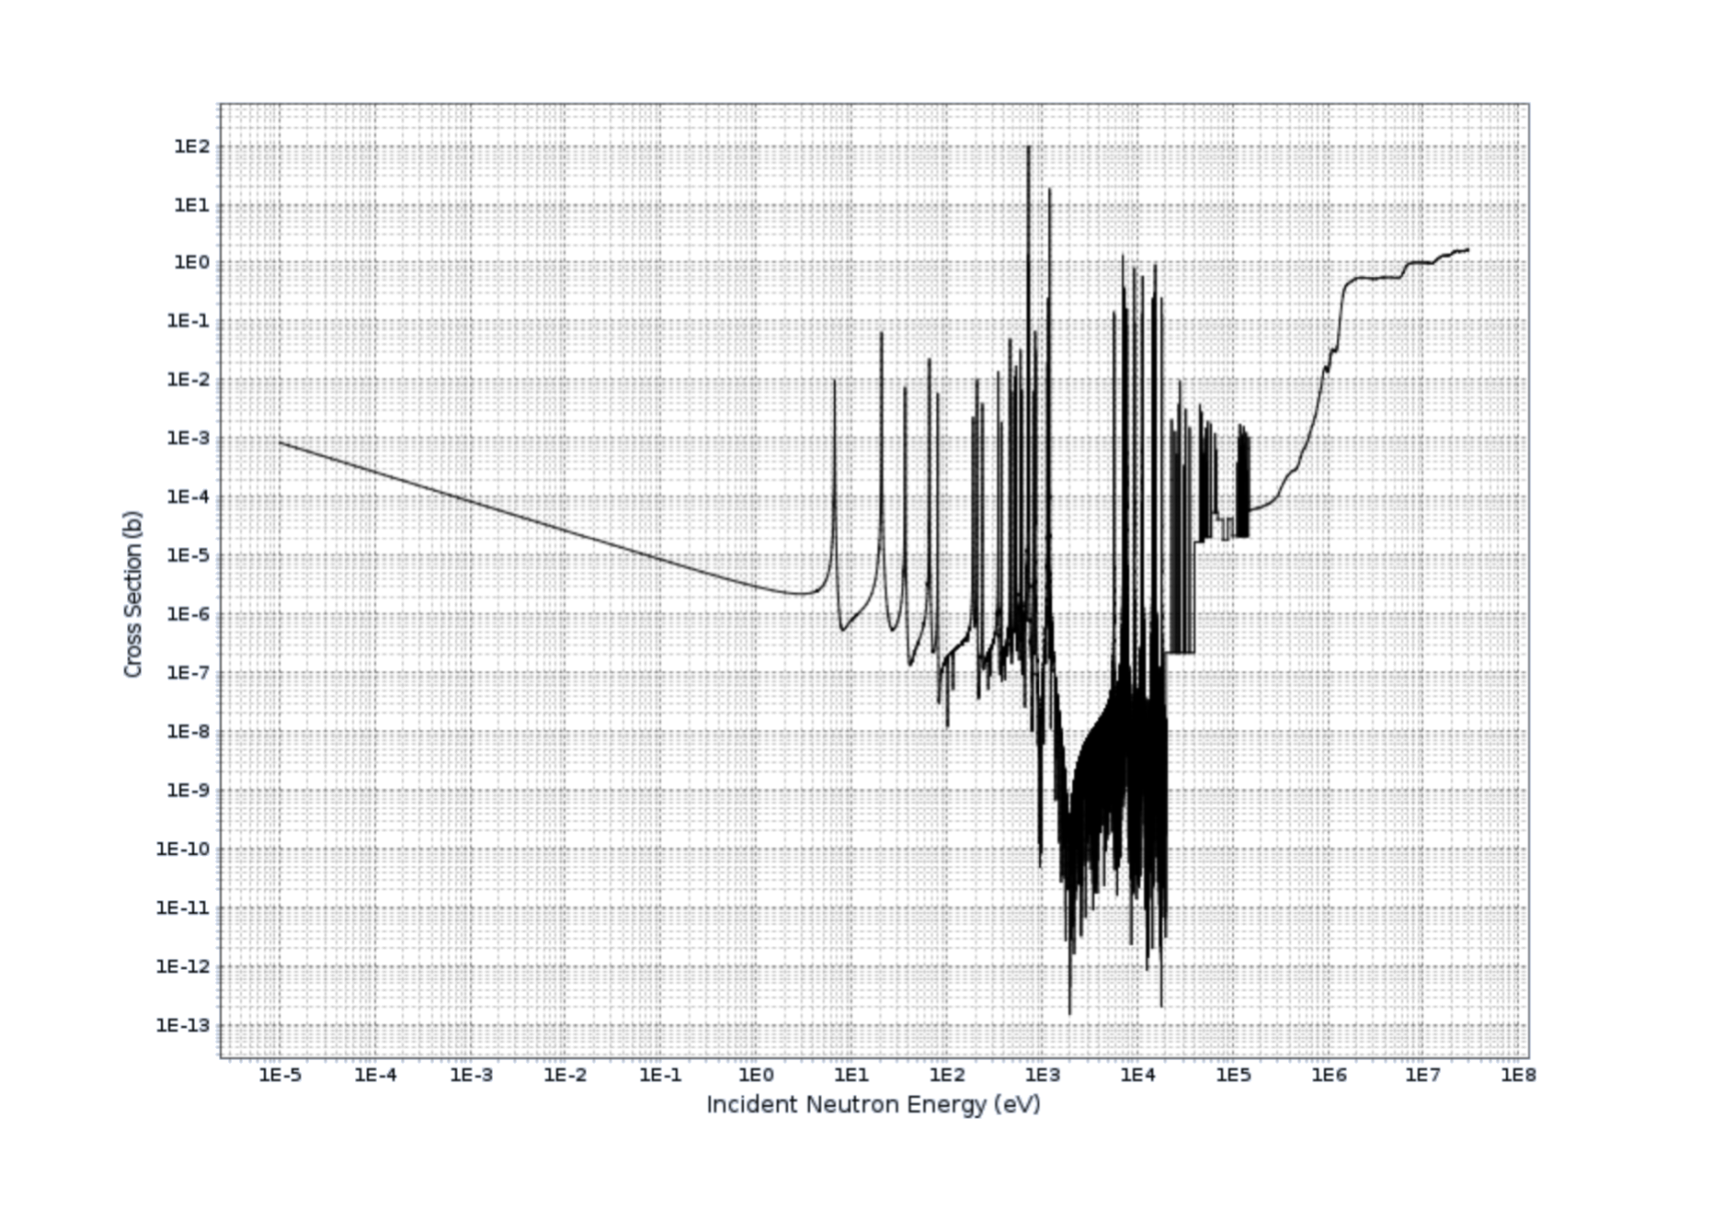
\includegraphics[width=8cm]{u238_fission.png}
(b) 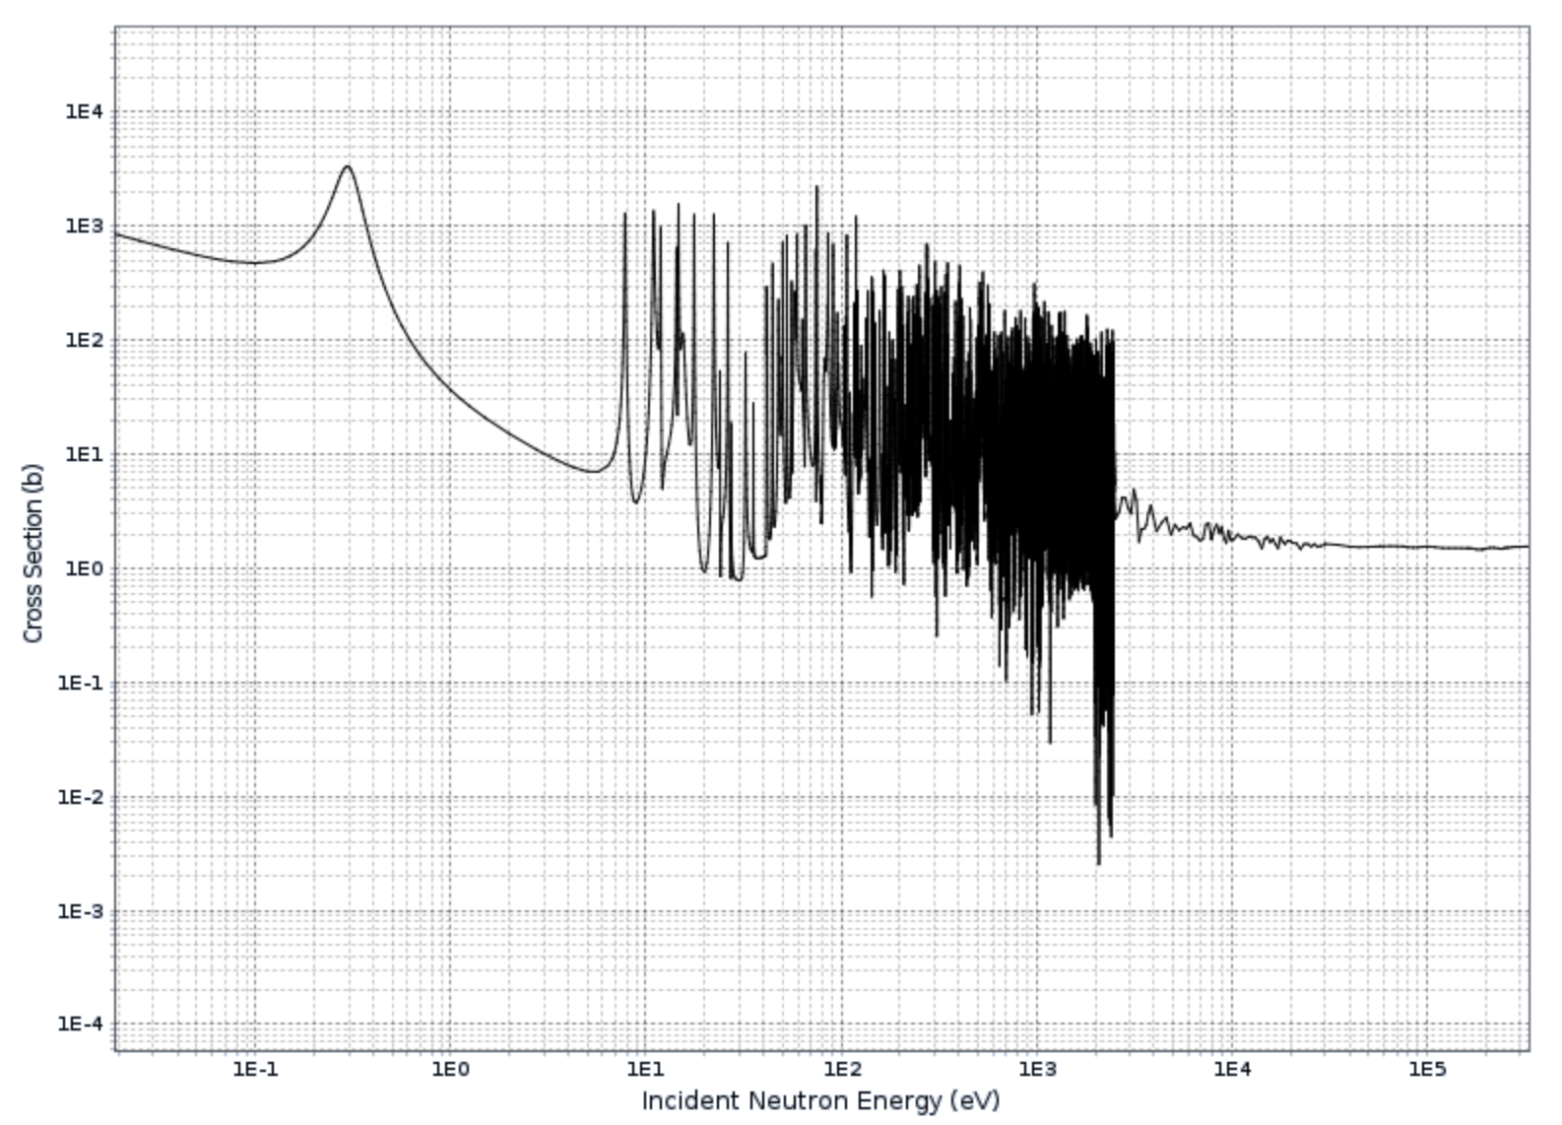
\includegraphics[width=8cm]{pu239_fission.png} \\
(c) 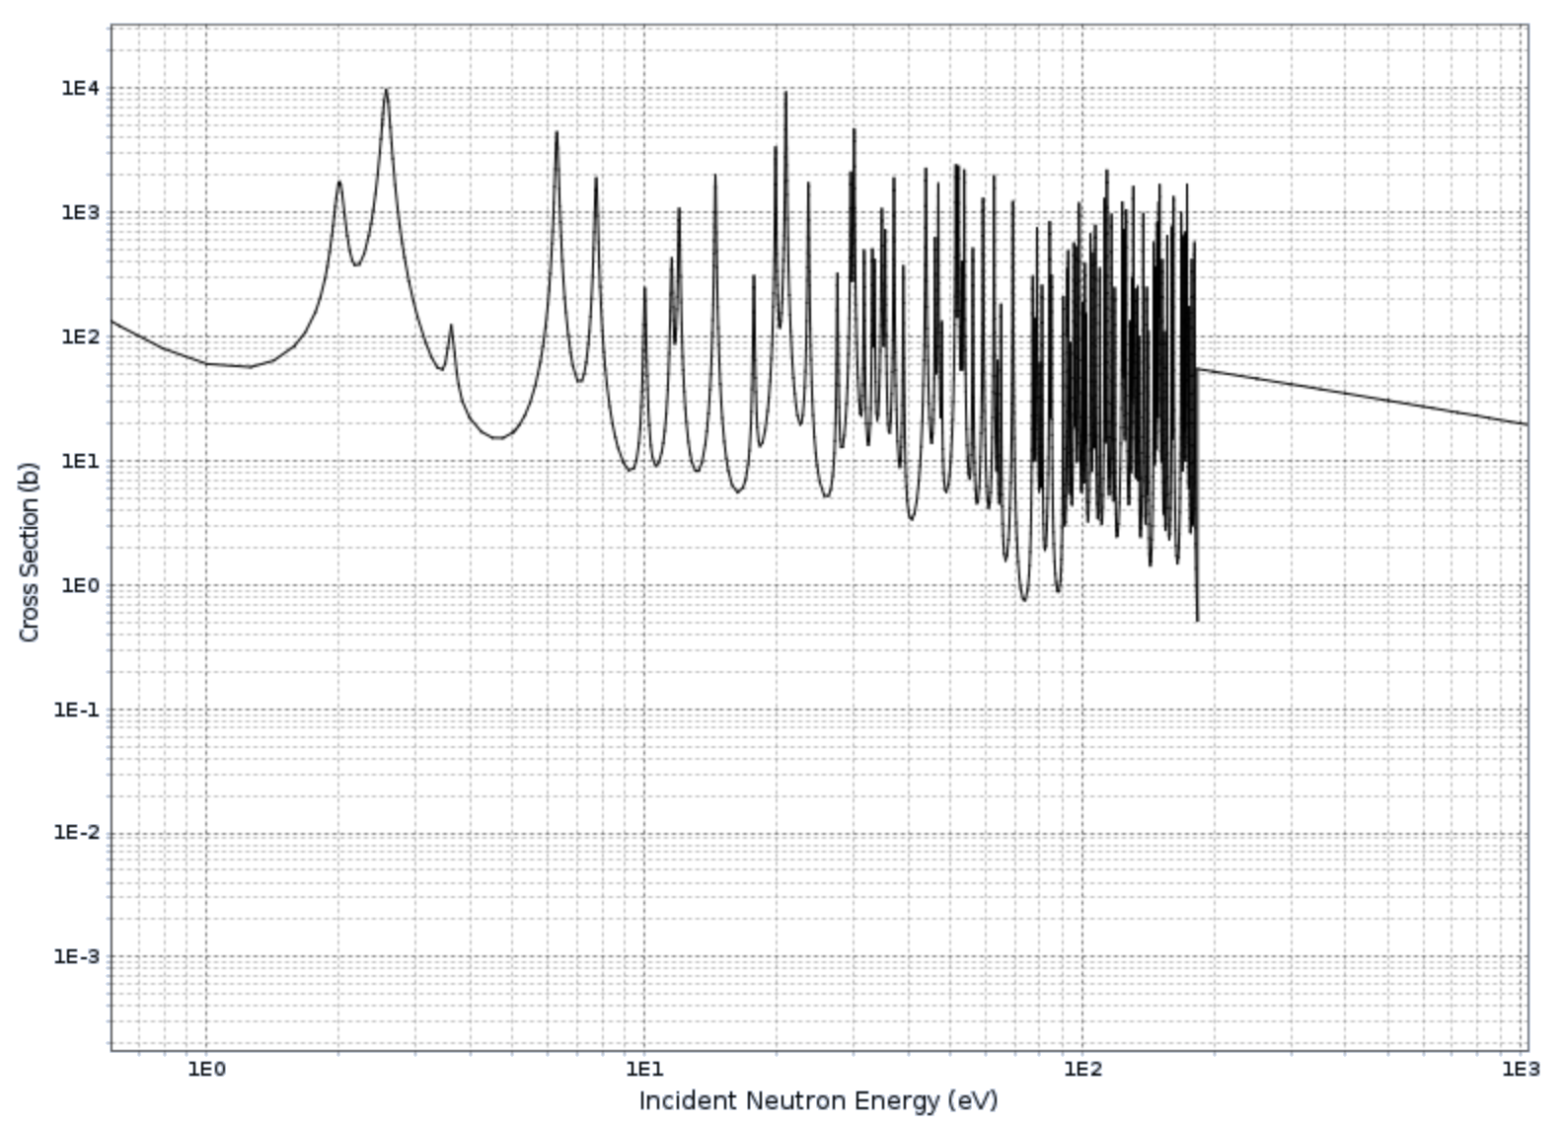
\includegraphics[width=8cm]{gd155_absorption.png}
(d) 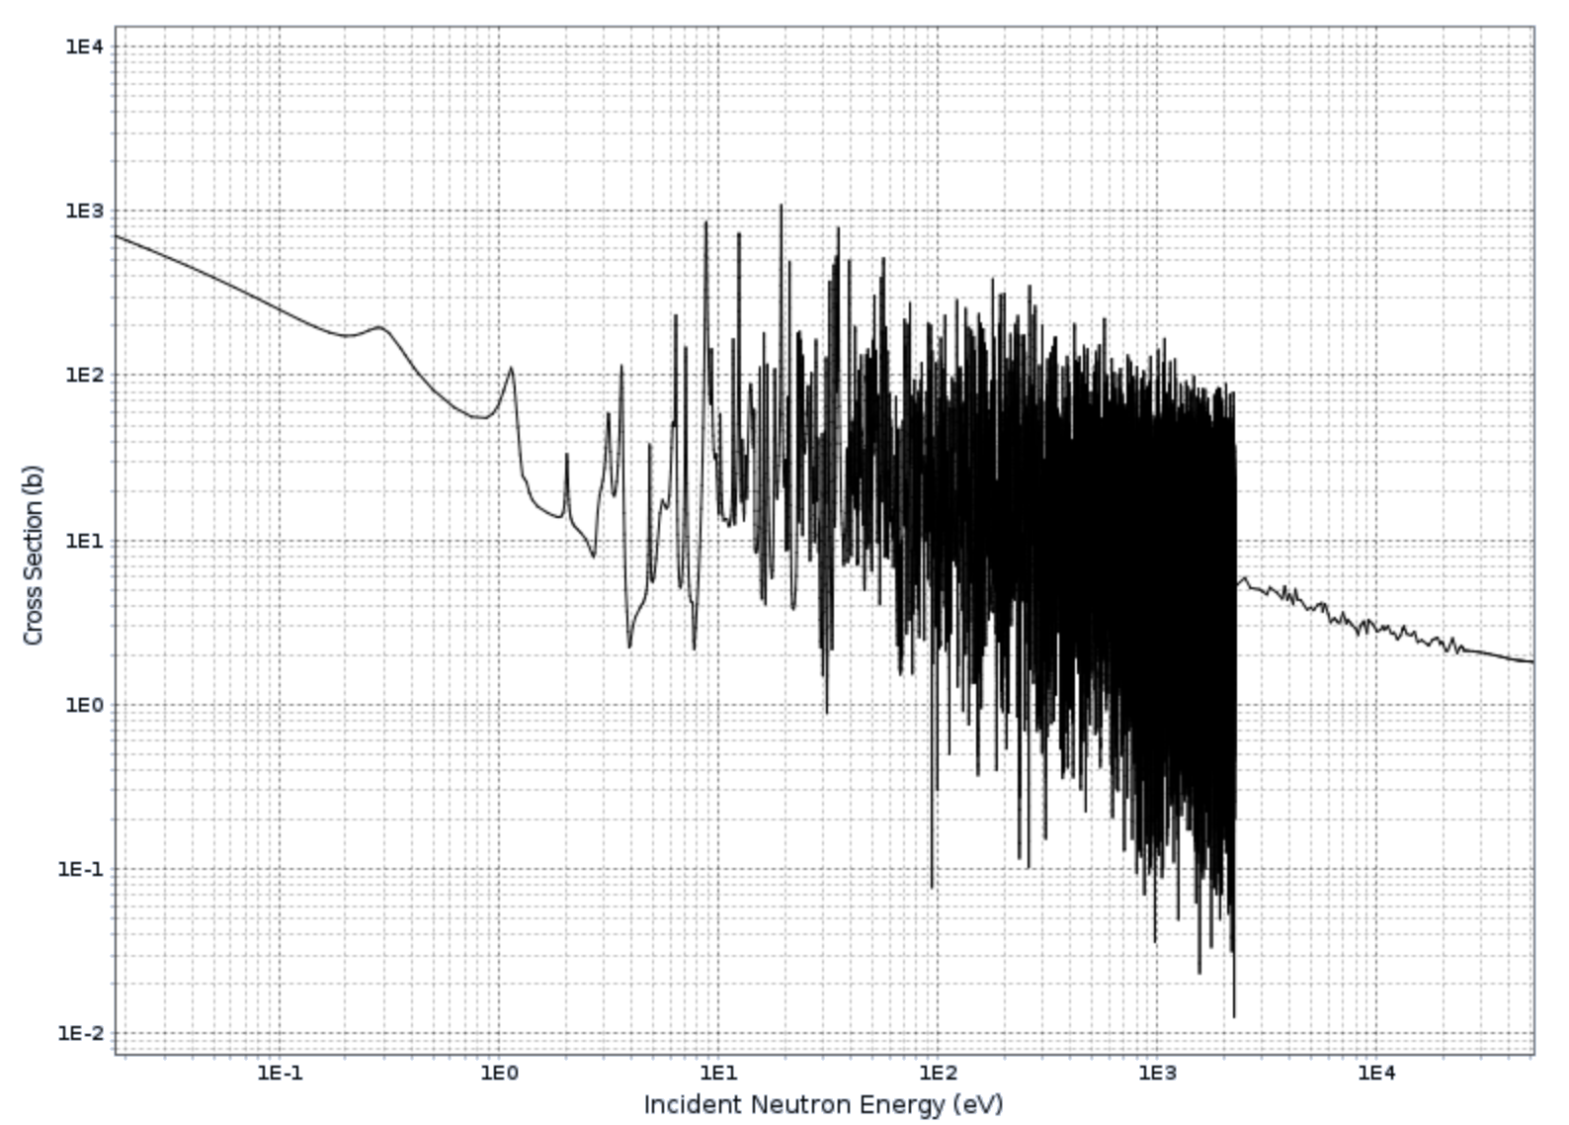
\includegraphics[width=8cm]{u235_fission.png}\\
(e) 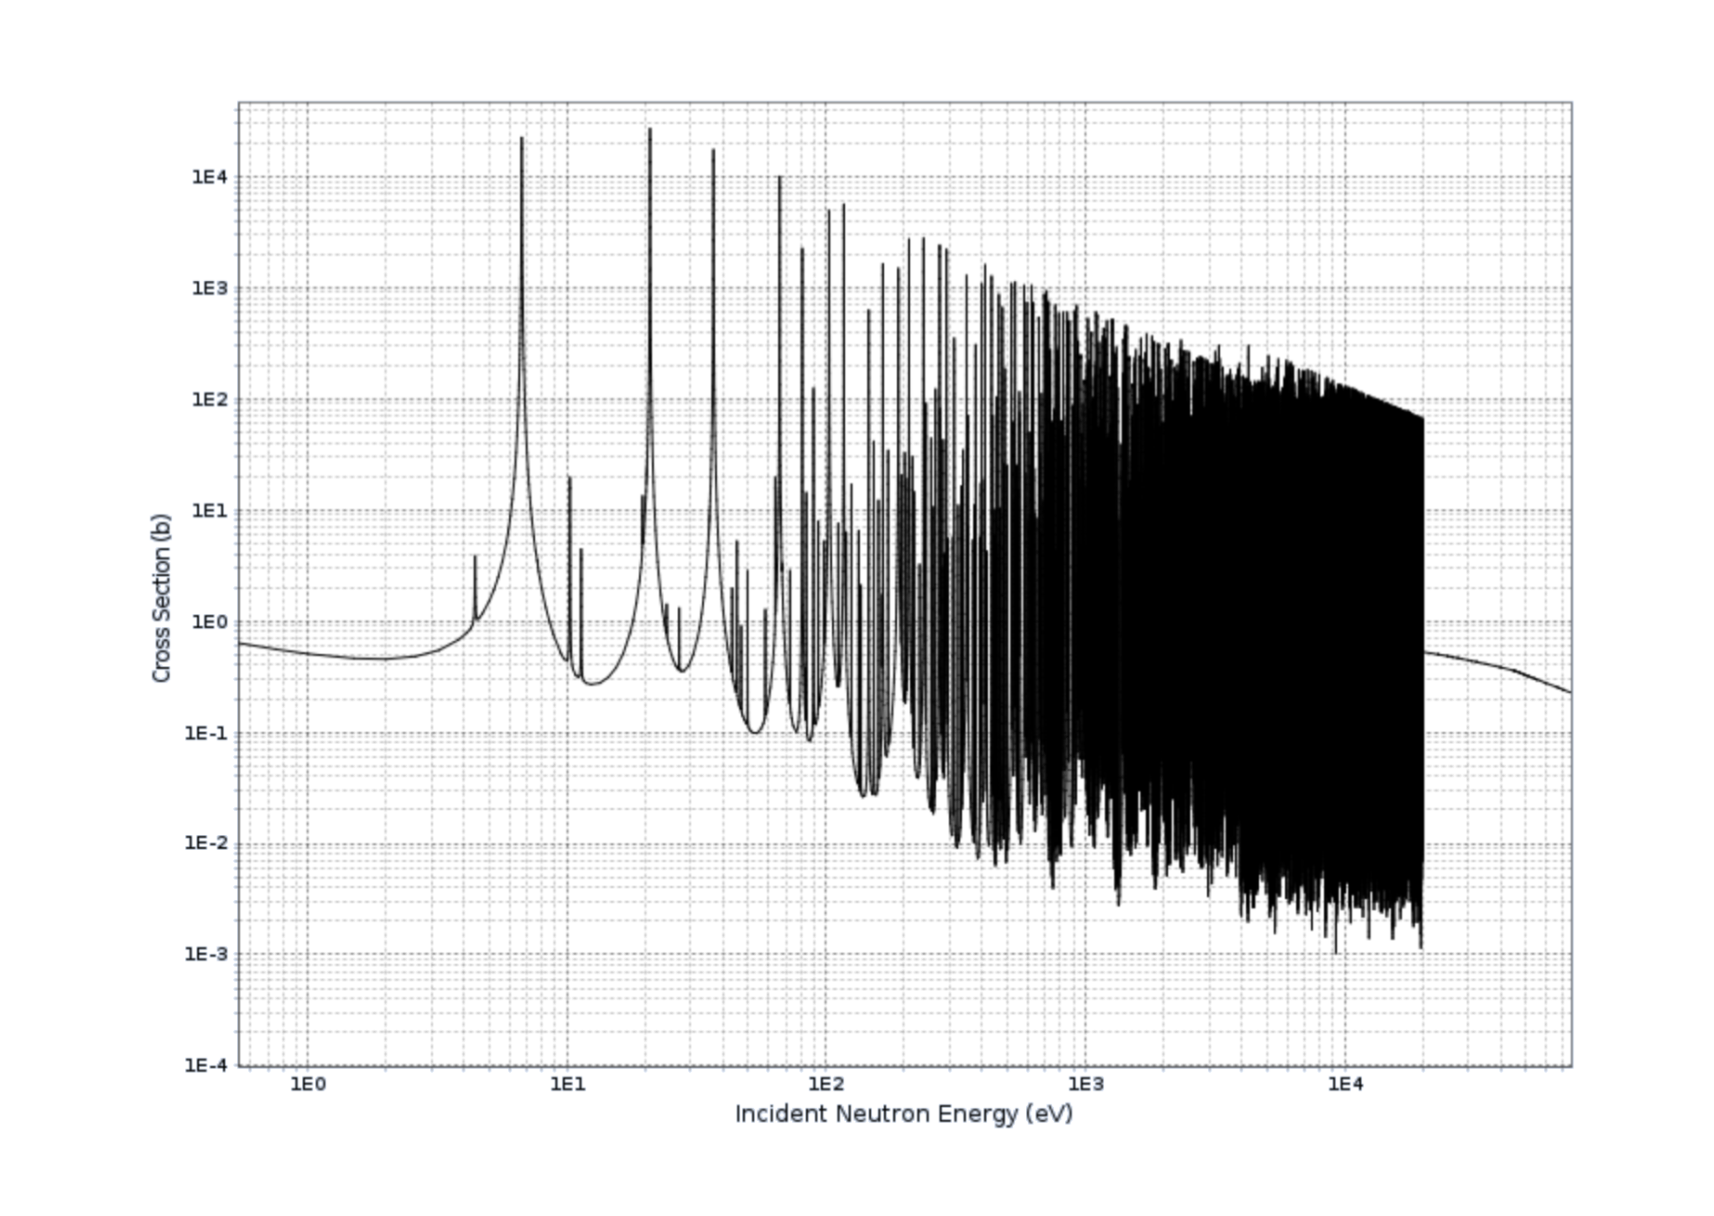
\includegraphics[width=8cm]{u238_absorption.png}



\section*{Problem 4 Solution}


\tab\tab (a) \, 4 \, $^{238}$U fission (high fast region) 					\\
\tab\tab (b) \, 5 \, $^{239}$Pu fission (resonance peak)					\\
\tab\tab (c) \, 1 \, $^{155}$Gd absorption (consistently high absorption)	\\
\tab\tab (d) \, 2 \, $^{235}$U fission (high thermal fission cross section)	\\
\tab\tab (e) \, 3 \, $^{238}$U absorption (large absorptive resonances)



\end{document}